\subsection{Cahn-Hilliard Simulations}

%%%%%%%%%%%%%%%%%%%%%%%%%%%%%%%%%%%%%%%%%%%%%%%%%%%%%%%%%%%%%%%%%%%%%
\royslide{Mesh Refinement}{

\begin{minipage}[h]{.45\textwidth}
\begin{center}
\includegraphics[width=.9\textwidth]{figs/chem-0250}
\end{center}
\end{minipage}
\begin{minipage}[h]{.45\textwidth}
\royitemizebegin{Coarse mesh}
\item $32 \times 32$ bicubic elements
\item $\Delta t = 2.500 \times 10^{-4}$
\item $t = 0.0625$
\item Mesh resolution must capture equilibrium interface width
\item Timesteps are limited by nonlinear solver
\royitemizeend
\end{minipage}

}


%%%%%%%%%%%%%%%%%%%%%%%%%%%%%%%%%%%%%%%%%%%%%%%%%%%%%%%%%%%%%%%%%%%%%
\royslide{Mesh Refinement}{

\begin{minipage}[h]{.45\textwidth}
\begin{center}
\includegraphics[width=.9\textwidth]{figs/chem-0500}
\end{center}
\end{minipage}
\begin{minipage}[h]{.45\textwidth}
\royitemizebegin{One Refinement}
\item $64 \times 64$ bicubic elements
\item $\Delta t = 1.250 \times 10^{-4}$
\item $t = 0.0625$
\item Free energy decay limits most error growth
\item Primary exception: interface topology changes
\royitemizeend
\end{minipage}

}

%%%%%%%%%%%%%%%%%%%%%%%%%%%%%%%%%%%%%%%%%%%%%%%%%%%%%%%%%%%%%%%%%%%%%
\royslide{Mesh Refinement}{

\begin{minipage}[h]{.45\textwidth}
\begin{center}
\includegraphics[width=.9\textwidth]{figs/chem-1000}
\end{center}
\end{minipage}
\begin{minipage}[h]{.45\textwidth}
\royitemizebegin{Two Refinements}
\item $128 \times 128$ bicubic elements
\item $\Delta t = 0.625 \times 10^{-4}$
\item $t = 0.0625$
\item Finite Element error becomes negligible
\item Uncertainty issues remain
\royitemizeend
\end{minipage}

}

%%%%%%%%%%%%%%%%%%%%%%%%%%%%%%%%%%%%%%%%%%%%%%%%%%%%%%%%%%%%%%%%%%%%%
\royslide{Mesh Refinement}{

\begin{minipage}[h]{.55\textwidth}
\begin{center}
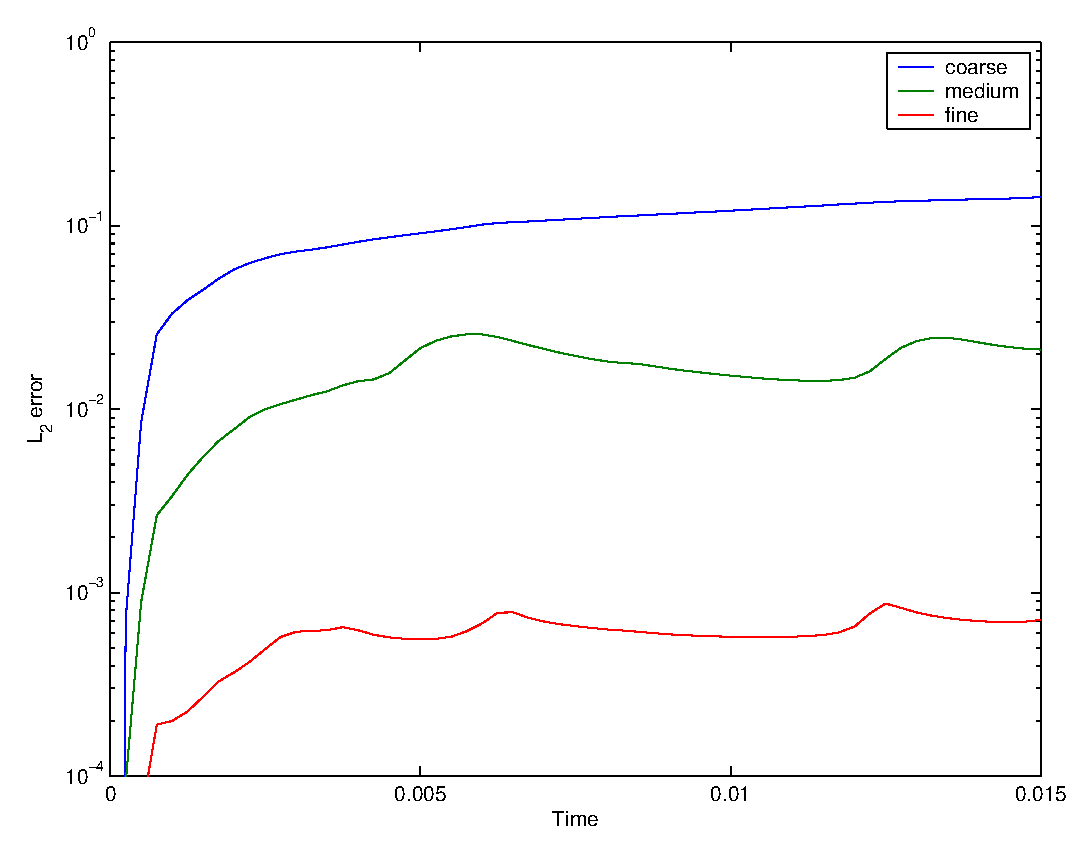
\includegraphics[width=.9\textwidth]{figs/cherror}
\end{center}
\end{minipage}
\begin{minipage}[h]{.4\textwidth}
\royitemizebegin{Transient Error}
\item With layers well-resolved, error remains bounded
\royitemizeend
\end{minipage}

}



%%%%%%%%%%%%%%%%%%%%%%%%%%%%%%%%%%%%%%%%%%%%%%%%%%%%%%%%%%%%%%%%%%%%%
\royslide{Adaptive Time Stepping}{

\begin{columns}
\begin{column}{.55\textwidth}
\begin{center}
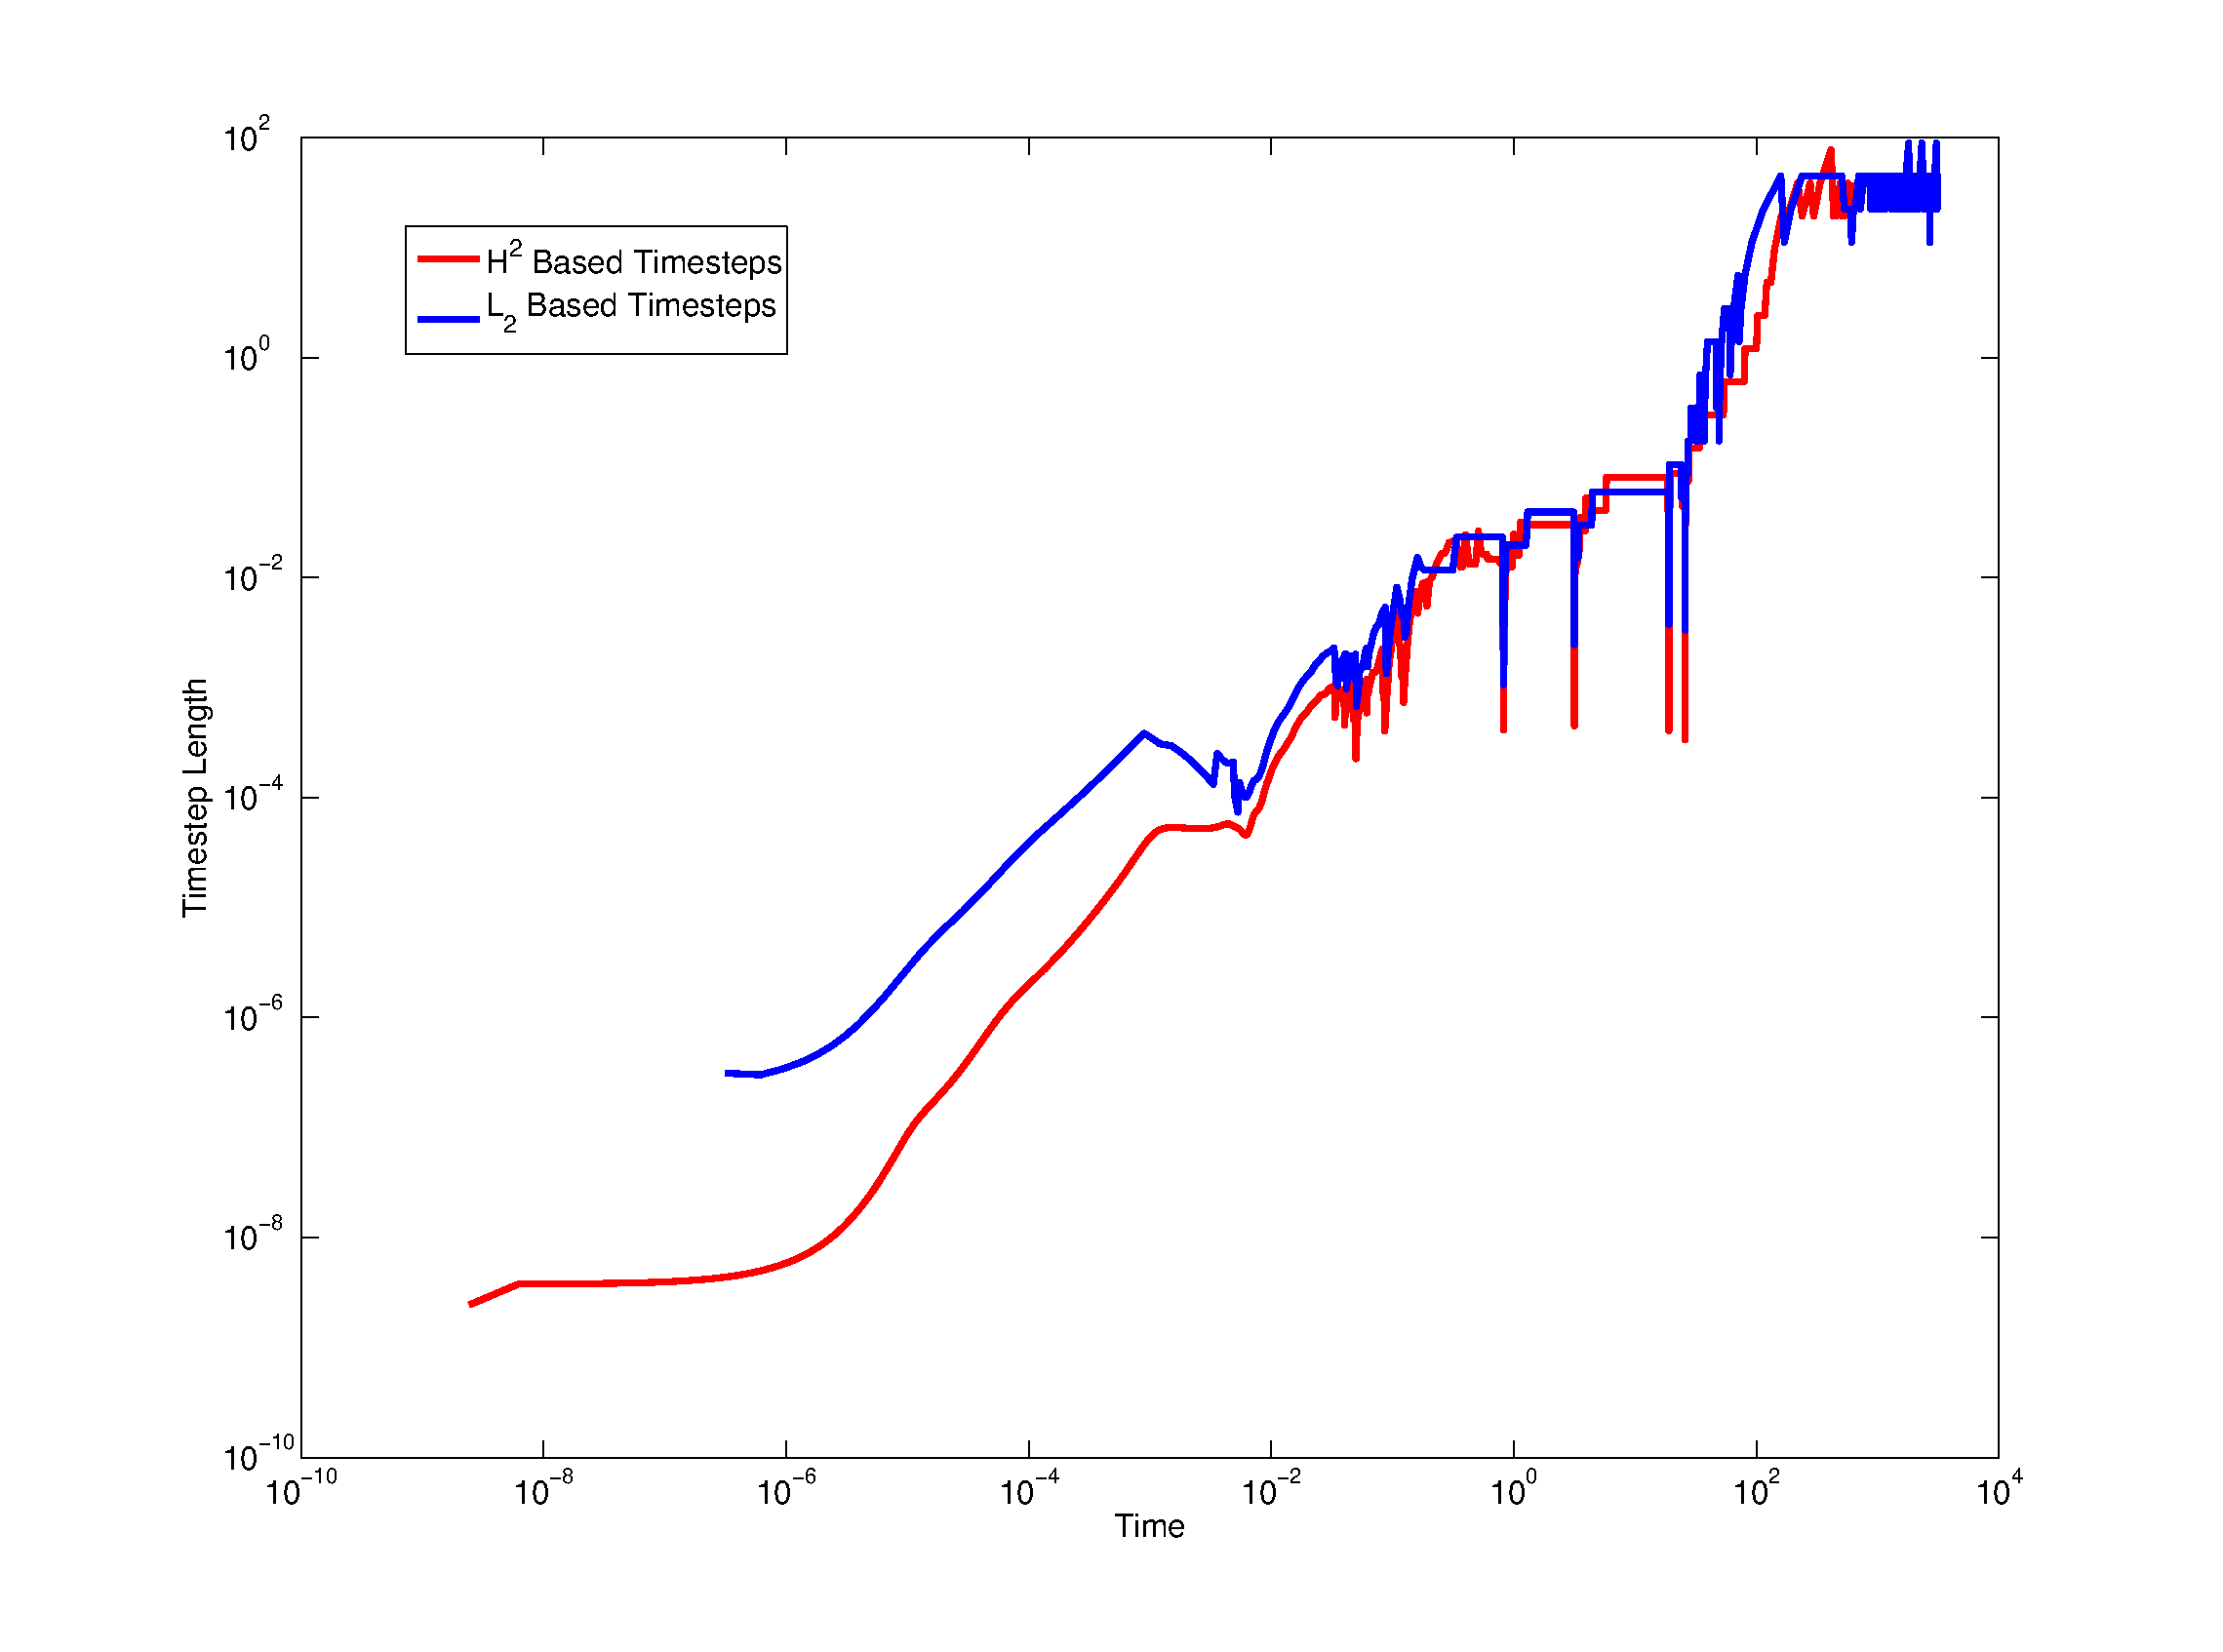
\includegraphics[width=.9\textwidth]{figs/adaptivetimesteps}
\end{center}
\end{column}
\begin{column}{.45\textwidth}
\royitemizebegin{}
\item CahnHilliardSystem
\item Euler2Solver
\item AdaptiveTimeSolver
\item Orders of magnitude speedup
\royitemizeend
\end{column}
\end{columns}

}



%%%%%%%%%%%%%%%%%%%%%%%%%%%%%%%%%%%%%%%%%%%%%%%%%%%%%%%%%%%%%%%%%%%%%
\royslide{Phase Separation - Spinodal Decomposition}{

\royitemizebegin{Initial Evolution}
\item Initial homogeneous blend quenched below critical T
\item Random perturbations rapidly segregate
into two distinct phases, divided by a labyrinth of sharp interfaces
\item Rapid anti-diffusionary process
\royitemizeend

\begin{center}
\includegraphics[width=.3\textwidth]{figs/ch3D02-006}
\includegraphics[width=.3\textwidth]{figs/ch3D02-012}
\includegraphics[width=.3\textwidth]{figs/ch3D02-024}
%\includegraphics[width=.3\textwidth]{figs/ch010}
%\includegraphics[width=.3\textwidth]{figs/ch050}
%\includegraphics[width=.3\textwidth]{figs/ch100}
\end{center}
}


%%%%%%%%%%%%%%%%%%%%%%%%%%%%%%%%%%%%%%%%%%%%%%%%%%%%%%%%%%%%%%%%%%%%%
\royslide{Phase Separation - Interfacial Flow}{

\royitemizebegin{Long-term Evolution}
\item Single-phase regions gradually coalesce
\item Motion into curvature vector resembles surface tension
\item Patterning may occur when additional stress, surface tropisms
are applied
\royitemizeend

\begin{center}
\includegraphics[width=.3\textwidth]{figs/ch3D02-048}
\includegraphics[width=.3\textwidth]{figs/ch3D02-096}
\includegraphics[width=.3\textwidth]{figs/ch3D02-192}
%\includegraphics[width=.3\textwidth]{figs/ch100}
%\includegraphics[width=.3\textwidth]{figs/ch200}
%\includegraphics[width=.3\textwidth]{figs/ch500}
\end{center}

}
